\clearpage

\section{Opaque with 1+1 Protection}
In this case study we focus on the opaque case with 1 + 1 protection.

\subsection{Physical Network Topology}

\subsubsection{Reference Network}
As we can see in the figure, our reference network consists of 6 nodes and 8 Bidirectional links.
The average length of the links was chosen so that the following calculations are more simplistic.

\begin{figure}[h!]
\centering
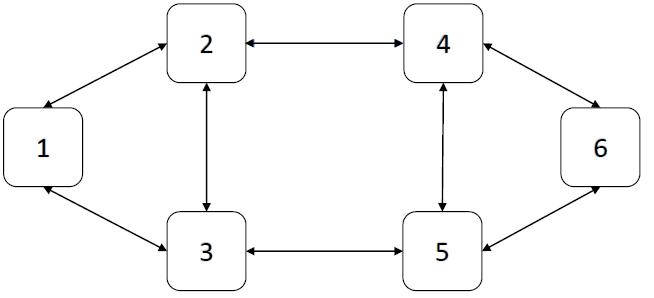
\includegraphics[width=\textwidth]{RedeTeste}
\caption{Physical Topology of the Reference Network.}
\end{figure}


The following table shows the values of the variables associated with this network.
\begin{table}[h!]
\centering
\begin{tabular}{|| c | c | c||}
 \hline
 Constant & Description & Value \\
 \hline\hline
 N & Number of Nodes & 6 \\
 L & Number of Bidirectional Links & 8 \\
 <$\delta$> & Node out-degree & 2,667 \\
 <len> & Mean Link Length (km) & 500 \\
 <h> & Mean Number of Hops,for Working Paths & 1,533 \\
 <h'> & Mean Number of Hops,for Backup Paths & 2,467 \\
 \hline
\end{tabular}
\caption{Table of reference network values}
\label{table:1}
\end{table}

As we can see from table \ref{table:1}, to do all the calculations necessary for this project, let us know the value of the traffic used. This value is defined depending on the scenario used, as we can see:
\begin{itemize}
  \item Low Traffic: \textbf{0.5 TBits/s}
  \item High Traffic: \textbf{5 TBits/s}
\end{itemize}

\subsubsection{Realistic Network}
The real network chosen for this work is the EON (European Optical Network).
The way the nodes are arranged geographically can be seen from the following figure.

\begin{figure}[h!]
\centering
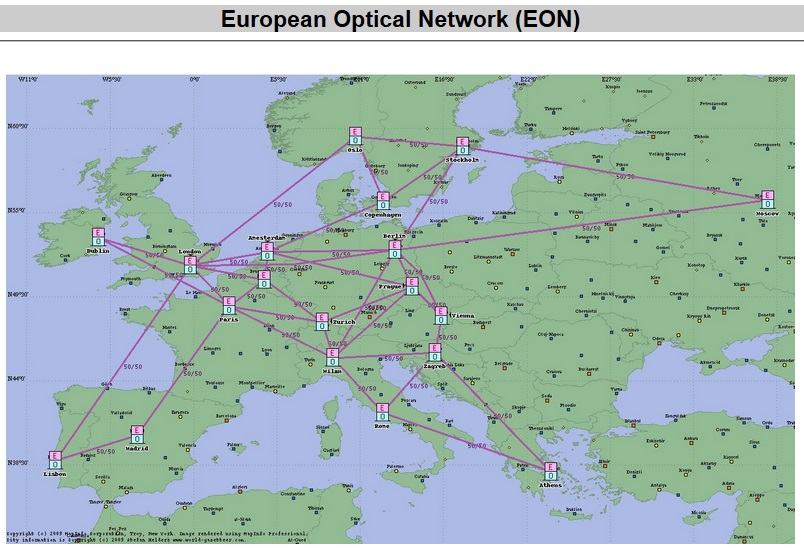
\includegraphics[width=\textwidth]{EON_Rede_Realista}
\caption{Physical Topology of the Realistic Network.}
\end{figure}

The table \ref{table:2} shows the values of the variables associated with this network.
\begin{table}[h!]
\centering
\begin{tabular}{|| c | c | c||}
 \hline
 Constant & Description & Value \\
 \hline\hline
 N & Number of Nodes & 19 \\
 L & Number of Bidirectional Links & 37 \\
 <$\delta$> & Node out-degree & 3,89 \\
 <len> & Mean Link Length (km) & 753,76 \\
 <h> & Mean Number of Hops,for Working Paths & 2,3 \\
 <h'> & Mean Number of Hops,for Backup Paths & 3,2 \\
 \hline
\end{tabular}
\caption{Table of realistic network values}
\label{table:2}
\end{table}

Again, to make all the necessary calculations, only the value of the traffic used is missing. This value is set depending on the scenario used, as we can see:

\begin{itemize}
  \item Low Traffic: \textbf{2 TBits/s}
  \item High Traffic: \textbf{20 TBits/s}
\end{itemize}

\subsection{Dimensioning using ILP models}

The objective function of following ILP is a minimization of the sum of two variables: total number of flows crossing link (i; j) for all demand pairs (o; d) and total number of optical channels in each link (i; j).
\begin{figure}[h!]
  \centering
  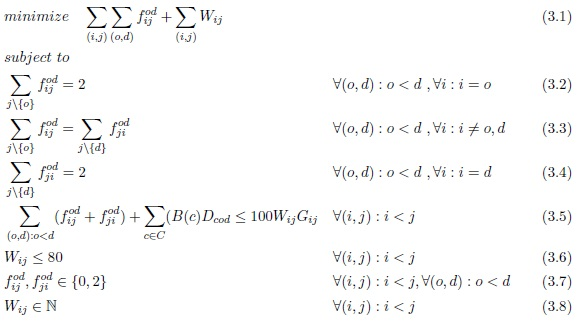
\includegraphics[scale=1]{ILP_Opaque}
\end{figure}

The objective function, to be minimized, is the expression(3.1). The flow conservation constraints are (3.2), (3.3) and (3.4). First constraint ensures that, for all demand pairs (o,d), it routes two flows of traffic for all bidirectional links (i,j) when "j" is not equal to the origin of the demand. Equation (3.4) is based on the same idea of (3.1), however applied in reverse direction. Assuming bidirectional traffic, so the number of flows in both directions of the link is the same (3.3). The inequality (3.5) is considered grooming constraint, so it means the total client traffic flows can not be greater than the capacity of optical channels on all links. Another important constraint (3.6) is the capacity of the optical channels which must be less or equal to 100 Gb/s or 80 ODU0. The number of flows per demand can be zero if there are no traffic demands or two if considering working and protection traffic (3.7). The last constraint is just needed to ensure the number optical of channels is a positive integer values greater than zero.


\subsection{ILP Results}
In this initial phase the results will be presented using ILP to calculate the CAPEX of the reference network.
For this we will use the following calculation formulas:

\begin{figure}[h!]
  \centering
  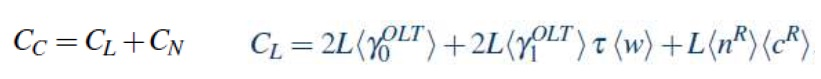
\includegraphics[width=\textwidth]{CAPEX}
  \caption{First function is CAPEX cost, second is cost of the links}
\end{figure}

\begin{figure}[h!]
  \centering
  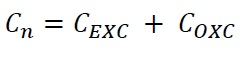
\includegraphics[scale=1]{CAPEX2}
  \caption{This function represent the cost of the nodes}
\end{figure}

We will also need a price list that we can see below.

\begin{figure}[h!]
  \centering
  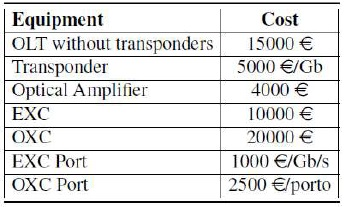
\includegraphics[scale=1]{TabValor}
  \caption{Table with costs}
\end{figure}

Finally we will calculate the CAPEX values for the various situations mentioned.

First we will present the scenario of low traffic and then in the case of a high of traffic.
To know the value of CAPEX we will have to first calculate the value of the cost of the links and then the cost of the nodes.

\textbf{First scenario:}

Through the table, of auxiliary calculations and MatLab the value of the cost of the links is:

Cost link = 24 336 000 euros

Again, through the table, of auxiliary calculations and MatLab the value of the cost of the nodes is:

Cost node = 5 860 000 euros

Finally, for this scenario the cost of CAPEX is:

CAPEX = 30 196 000 euros

\textbf{Second scenario:}

Cost link = 191 336 000 euros

Cost node = 48 260 000 euros

CAPEX = 239 596 000 euros


\subsection{Heuristics}

